\documentclass{sig-alternate}
\usepackage{subfigure}
\usepackage{amssymb,amsmath}
\sloppy
%
\usepackage{makeidx}  % allows for indexgeneration
\usepackage{graphicx}        % standard LaTeX graphics tool
                             % when including figure files

\usepackage{multicol}        % used for the two-column index
\usepackage[bottom]{footmisc}% places footnotes at page bottom
\usepackage{amsmath,epsfig}
\usepackage{algorithm}
\usepackage{algorithmic}
\usepackage{subfigure}
\usepackage{multirow}
\usepackage{url}


\begin{document} % Something about unreliable workers: assessing the effect, for instance - JJ
\title{ Randomized Parameter Settings for Heterogeneous Workers in a Pool-Based Evolutionary Algorithm}
\subtitle{TRACK: }

\conferenceinfo{GECCO'14,} {July 12-16, 2014, Vancouver, BC, Canada.}
    \CopyrightYear{2014}
    \crdata{TBA}
    \clubpenalty=10000
    \widowpenalty = 10000
% --- End of Author Metadata ---

%
%\titlerunning{Unreliable Heterogeneous Workers in EvoSpace}  % abbreviated title (for running head)
%                                     also used for the TOC unless
%                                     \toctitle is used
%
%\author{
%\alignauthor Leonardo Trujillo,   \\
%             Enrique Naredo\\
%       \affaddr{TREE-LAB, Doctorado en Ciencias de la Ingenier\'ia}\\
%       \affaddr{Instituto Tecnol\'ogico de Tijuana}\\
%       \affaddr{Tijuana, B.C., M\'exico}\\
%       \affaddr{Web: www.tree-lab.org} \\ 
%       \affaddr{enriquenaredo@gmail.com}\\
%       \affaddr{leonardo.trujillo@tectijuana.edu.mx}\\
%}

\maketitle              % typeset the title of the contribution

\begin{abstract}
%Abstract is important and should go first.
Several pool-based Evolutionary Algorithms (EAs) have been proposed that asynchronously distribute the evolutionary process among heterogeneous devices, not only among controlled nodes but also in those outside the data center, in web browsers or cloud based virtual machines. This reach out approach allows researchers the use of low cost computational power not available otherwise, but on the other hand, have the challenge to manage heterogeneous and unreliable computing resources. In these algorithms the population is stored in a shared pool where distributed processes called Workers execute the actual evolutionary process. The performance of these algorithms depends in part on having proper parameter settings for the GA executed in each worker along with the overall configuration. Parameter settings may include: sample size, generations, mutation rate and crossover rate. In this paper we evaluate a strategy proposed by Gong and Fukunaga for the Island-Model which statically assigns random control parameter values to each worker. Experiments were conducted to assess the performance of this strategy on pool-based EAs using benchmark problems and the EvoSpace framework. The results suggest that this approach can yield results which are competitive to instances of the algorithm using Workers with control parameters tuned specifically for the benchmark. 
\end{abstract}

% A category with the (minimum) three required fields
\category{I.2.2}{Artificial Intelligence}{Automatic Programming}[program synthesis]

\terms{Performance,Theory,Experimentation}
\keywords{}

\section{Introduction}
\label{sec:intro}
Thanks in part  to evolutionary computation (EC) research, scientists and engineers from many fields now understand the remarkable power of
the natural search process described by the biological theory of Neo-Darwinian evolution \cite{holland}. 
Inspired in biological evolution, EC researchers have developed a variety of search and optimization algorithms \cite{eiben}.
%Empty statement, maybe delete.

While EAs are inspired by evolution, they mostly follow an abstract model of the natural process.
For instance, one aspect that is omitted from most EAs is an open-ended search process,
in practice EAs are used to solve problems with well defined objectives, while natural evolution is an adaptive process without an a priori goal or purpose.
Such open-ended EAs have been developed, mostly for artistic design \cite{Musart}, interactive evolution \cite{ie1} and artificial life systems \cite{avida}.
Other interesting features of biological evolution, is that it is an intrinsically parallel, distributed and asynchronous process,
undoubtedly important features that have allowed evolution to produce impressive results throughout nature.
However, some of these features are not trivially included into standard EAs,
which are mostly coded as sequential and synchronous algorithms \cite{eiben}.

For instance, a large body of work exists in EA parallelization, using multiple CPU cores, multiple nodes and GPUs \cite{}.
However, distributed and asynchronous EAs have started to become common only recently.
In particular, recent trends in information technology have opened new lines of future development for EC research.
Today, computing resources computing power range from personal computers and smart-devices to massive data centers.
These resources are easily accessible through popular Internet technologies, such as cloud computing, 
peer-to-peer (P2P), and web environments.

Moreover, these technologies are intended for the development of parallel, distributed and asynchronous systems,
such that an EA developed on top of them could easily reap the benefits of these features.
As stated before, several EAs have been proposed that distribute  the evolutionary process among heterogeneous devices, not only among controlled
nodes within an in-house cluster or grid, but also to others outside the data center, in users' web browsers, smart phones or external cloud based virtual machines.
This reach out approach allows researchers to use low cost computational 
power that would not be available otherwise, but on the other hand, have the 
challenge to manage heterogeneous unreliable computing resources. 
In particular, we are interested in systems that follow a pool-based approach, where the search process is conducted
by a collection, of possibly heterogeneous, collaborating processes using a shared repository or population pool.
We will refer to such algorithms as Pool-based EAs or PEAs, and highlight the fact that such systems are
intrinsically parallel, distributed and asynchronous.

Despite promising results, PEAs present several notable challenges. From a technological perspective, for example, lost 
connections, low bandwidth, abandoned work, security and privacy are all important issues that must be addressed. 
However, here we focus on a common issue with most EAs, that is only amplified in a PEA, a problem that can be referred to as parametrization.
In general, among machine learning methodologies, EAs are highly criticized by the large number of parameters they posses,
that for real world problems need to be tuned empirically or require additional heuristic processes to be included into the search to
adjust the parameters automatically \cite{ss}.
In the case of a PEAs, this issue is magnified since the underlying system architecture adds several degrees of freedom to the search process.

This work studies a recently proposed pool-based system called EvoSpace, a framework to develop PEAs using 
a heterogeneous collection of possibly unreliable resources.
EvoSpace is based on Linda's tuple space coordination model, where each node asynchronously
pulls its work from a central shared memory  \cite{Evospace,Musart,FreeLunch,Fire}. The core elements of EvoSpace are a central 
repository for the evolving population and remote clients here called EvoWorkers
which pull random samples of the population to perform on them the basic evolutionary
processes (selection, variation and survival), once the work is done, the
modified sample is pushed back to the central population.
Despite some promising initial results \cite{Evospace,Musart,FreeLunch,Fire}, research devoted to EvoSpace has not addressed the parametrization issue mentioned above.
In the study presented here, a recent approach called Randomized Parameter Setting Strategy (RPSS) \cite{fuku1,fuku2} is applied to EvoSpace and tested on several
benchmark problems.
The idea behind RPSS is that in a distributed EA, algorithm parametrization may be completely skipped for a successful search,
with research showing that when the number of distributed process is large enough, algorithm parameters can be set randomly and still achieve
good overall results.
However, work on RPSS has only focused on the well-known Island Model for EAs, a distributed but synchronous system.
% En el paper le llaman Distributed Island Model, para diferenciarla por ejemplo de Parallel Island Model en una maquina multiprocesador -Mario
% Pero, creo que lo distribuido no cambia el modelo, solo la implementacion, en el otro articulo si se refieren a el como Island Model ... tal vez si le ponemos (distibuted) Island Model ?
On the other hand, the goal of this work is to evaluate RPSS on a complete PEA implemented through EvoSpace.


%In this paper the effect of node unavailability in algorithms using the 
%EvoSpace population storage is assessed.   %Aquí aparece un
%                                %espacio muy grande en el PDF... - JJ
%
%This work evaluates the effect 
%of the re-insertion algorithm has on the total running time and number of evaluations 
%of a genetic algorithm. Using  a benchmark problem from the P-Peaks 
%problem generator, we compare both approaches: (i) the re-insertion previous
%individuals at the cost of keeping copies of samples, and (ii) inserting  
%randomly generated individuals, with the sometimes beneficial cost of 
%adding diversity to the population. For this experiments we use the same
%parameters used in an earlier work, in order to compare the 
%performance of the algorithm in similar conditions.
%EvoSpace was implemented as a web service on the popular Heroku platform 
%and EvoWorkers where simulated using PiCloud, a scientific computing PaaS. 

The remainder of the paper proceeds as follows. Section \ref{sec:work} 
%reviews related work. Afterwards, Section \ref{sec:evo} briefly describes the
%proposed EvoSpace framework and gives implementation details the re-insertion
%process. The experimental work is presented in Section \ref{sec:experiments}.
%Finally, a summary and concluding remarks are in Section \ref{sec:conclusions}.

\section{Related Work}
\label{sec:work}
Given the computational cost of many EAs, researchers have turned towards Internet and cloud based software systems.
For instance, Fern\'andez et al. \cite{nc}% articulo Paco, Gustavo y Leo publucado en Natural Computing}
use the well-known Berkeley Open Infrastructure for Network Computing (BOINC) to distribute EA runs across a
heterogeneous network of volunteer computers using virtual machines.

However, such a system, as well as others distributed or parallel systems, does not follow the PEA approach studied in the current paper.
In general, a pool-based system employs a central repository (real or virtual) where the evolving population is stored.
Distributed clients interact with the pool, performing some or all of the basic EA processes (selection, genetic operators, survival). 
For example, Smaoui et al. \cite{FekiNG09} uses BOINC redundancy
to deal with the volatility of nodes and unreliability of their results. 
In this work each BOINC work unit consisted of a fitness evaluation task and
multiple replicas were produced and sent to different clients, later when 
outputs were received a validation step ensured all outputs match.

Merelo et al. \cite{JSON} developed a Javascript PEA that distributes the evolutionary process over the web,
this provides the added advantage of not requiring the installation of additional software in each computing node. 
In this work the server receives an Ajax request with the best individual 
obtained from the local evolution in clients, and then responds with 
additional parameters and the best individual in the population so far. 
Other similar cloud-based solutions are based on a global queue of tasks and a Map-Reduce 
implementation which normally handles failures by the re-execution of  tasks \cite{fazenda2012,di2013towards,FlexGP}. 

%This should be expanded a bit

%% Los de abajo son comentarios viejos -Mario
%% Lo que hice arriba es ir comparando la técnica de failover de cada
%% propuesta me faltan las de abajo 

In general, this pool-based approach can be traced back to the A-Teams system \cite{ateam}, which is not restricted to evolutionary algorithms.
Another proposal is made by G. Roy et al. \cite{roy:2009}, who developed a multi-threaded system with a shared memory architecture that is
executed within a distributed environment and achieves substantial performance gains compared to standard approaches. On the other hand, Bollini and Piastra \cite{bollini:1999} emphasize persistence over performance, proposing a system that decouples population storage from the basic evolutionary operations. A similar decoupled model is proposed by Merelo et al. \cite{merelo:2008}, who used a database to store the population that is accessed through a web-server. Finally, a recent PEA is SofEA proposed by Merelo et al. \cite{sofea1,sofea2},
an EA that is mapped to a central CouchDB object store. It provides an asynchronous and distributed search process, where the four main evolutionary operators are decoupled from the evolving population.

This work, however, focuses on EvoSpace, a framework to develop PEAs using heterogeneous and unreliable resources \cite{Evospace,Musart,FreeLunch,Fire}, described in greater
detail in the following section.
 
\section{EvoSpace}
\label{sec:evo}
EvoSpace is based on Linda's tuple space \cite{Evospace} coordination model, where each node asynchronously
pulls its work from a central shared memory. The core elements of EvoSpace are a central 
repository for the evolving population and remote clients called EvoWorkers,
which pull random samples of the population to perform on them the basic evolutionary
processes (selection, variation and survival), once the work is done, the modified sample is pushed back to the central population.

This model contrasts with the use of a global queue of tasks and
implementations of map-reduce algorithms, favored in other proposals PEAs
\cite{fazenda2012,di2013towards,FlexGP}.
Following the tuple space model, when individuals are pulled from the EvoSpace
container these are removed from it, so that no other EvoWorker can use them.
This design decision has several known benefits relevant to concurrency control 
in distributed systems, and also is an effective way of distributing the workload.
Leaving a copy of the individual in the population server free to be pulled by other EvoWorkers will result in redundant work and this could be
costly if the task at hand is time consuming. EvoWorkers are expected to be 
unreliable, as they can loose a connection or are simply shut down or removed 
from the client. When an EvoWorker is lost, so are the individuals pulled from
the repository. Depending on the type of algorithm been executed, the lost of
these samples could have a high cost. To address the problem of unreliable 
EvoWorkers, EvoSpace uses a simple re-insertion algorithm that also 
prevents the starvation of the population pool. Other pool based algorithms
normally use a random insertion technique, but we argue this could negatively 
impact the outcome of the algorithm in some cases.



EvoSpace [{\em references hidden for blind review}] consists of two main components (see figure~\ref{fig:evo}): (i) the EvoSpace 
container that stores the evolving population and (ii) EvoWorkers, which execute 
the actual evolutionary process, while EvoSpace acts only as a population repository.
In a basic configuration, EvoWorkers pull a small random subset of the 
population, and use it as the initial population for a local EA executed 
on the client machine. Afterward, the evolved population from each EvoWorker 
is returned to the EvoSpace container. When individuals are pulled from the 
container they remain in a phantom state, they cannot be pulled again but 
they are not deleted. Only if and when the EvoWorker returns the replacement 
sample phantoms are truly deleted. If the EvoSpace container is at risk of 
starvation or optionally when a time-out occurs new phantom individuals are 
re-inserted to the population and available again. This can be done because a 
copy of each sample is stored in a priority queue used by EvoSpace to re-insert 
the sample to the central population; similar to games where characters are 
Re-spawned after a certain time. In the experiments conducted in this work 
re-insertion occurs when the population size is below a certain threshold. 
Figure~\ref{fig:evo} illustrates the main components of EvoSpace.

\begin{figure*}[t]
    \centering
        \includegraphics[width=5in]{eps/evospaceExample.eps}
    \caption{Main components and dataflow within EvoSpace.}
    \label{fig:evo}
\end{figure*}


\subsection{Implementation}
The population of an EA is stored in-memory using the key-value database Redis, chosen over a relational database system, or other non-SQL 
alternatives, because it provides a hash based implementation of sets  and queues which are natural data structures for a PEA model such as EvoSpace. 
EvoSpace is implemented as a python module and exposed as a web service using the Cherrypy HTTP library.
The EvoSpace modules are freely available with  a Simplified BSD License from \url{anonymous URL}.
% https://github.com/mariosky/EvoSpace. 

The EvoSpace system is deployed using Heroku, a multi-language Platform-as-a-Service (PaaS).
The basic unit of composition on
Heroku is a lightweight container running a single user-specified process.
These containers, which they call {\em dynos}, can include web (only these can receive {\tt http} requests) and worker processes
(including systems used for database and queuing, for instance).
Once deployed the web process can be scaled up by assigning more dynos;
in our case and in the more demanding configurations of our experiments, 
the web process was scaled to 20 dynos. Instructions and code for deployment 
is available at \url{anonymous URL}.
Finally, for the experiments carried out for this paper, EvoSpace workers are distributed using the PiClouf PaaS.

\section{Problem Statement}
As stated before, one of the main problems in EC research is referred to as parameter tuning.
This problem is of particular importance in real-world scenarios, where there can be little prior insights regarding what might be the best
configuration for an EA tool, especially if the intent is to use it as a black-box optimizer.
Indeed, this problem has received a growing level of interest in recent years, as evidenced by tracks such as Self-Search at GECCO,
where the aim is to develop self-adaptive or auto-tuning systems, that reduces the amount of human intervention that might be required before performing
an EA-based search.

However, recent work in \cite{fuku1,fuku2} has shown a promising alternate approach for EAs that employ multiple evolving populations.
In particular, the RPSS approach proposed in \cite{fuku1} is as interesting as it is simple.
First, consider the original configuration studied in \cite{fuku1,fuku2}, an Island Model EA.
In an Island Model, a set of N separate populations, or demes, run semi-isolated evolutionary processes, organized using a particular
neighborhood structure, such as ring or a random graph.
Each deme is not totally isolated, since after a certain amount of time (generations or function evaluation) a set of individuals is exchanged between
neighboring demes, a process known as migration.
Obviously, the problem of setting parameter values is magnified by a factor of N, since it is not possible to assume that for
a particular problem the best configuration is an homogeneous system where all demes share the same set of parameters.
Moreover, the additional complexity of the Island Model incorporates additional degrees of freedom that must be tuned before
performing a run.

Such a tuning task can become overwhelming, particularly if the number of islands is excessively large (hundreds).
Therefore, the proposal in \cite{fuku1} is to set the parameter values randomly, without a tuning or self-adaptive process whatsoever.
The RPSS approach is to set the parameters of each deme randomly at the beginning of the run, a very simple and apparently naive approach.
Nevertheless, results reported in \cite{fuku1,fuku2} exhibit promise, achieving competitive results while substantially reducing the amount
of effort required to tune the system (the approach only requires the user to specify a range of valid values for each parameter).

Following \cite{fuku1}, the proposal of the current work is to apply the RPSS approach to a PEA developed with EvoSpace.
However, before turning to the experimental work, lets highlight the main differences between a PEA and the Island Model studied in \cite{fuku1,fuku2}.
First, the Island Model is a synchronous EA, while it implements a higher level of parallelization than a normal EA, and is amenable to distributed implementations,
it still relies on a synchronized system in order to perform migration events.
Second, the PEA approach based on EvoWorkers can be implemented with as a more heterogeneous system than the Island Model.
In particular, the sample (population) size and number of generations executed by each EvoWorker can be different,
particularly since there is no need for synchronized migrations.
Notice that in EvoSpace, there is no explicit migration process, on the other hand EvoWorkers exchange population members through the centralized pool.
These differences could be important regarding the applicability of RPSS on an EvoSpace PEA,
which is evaluated in the experimental work presented next.



% Un comentario que hicieron en este paper es que perdemos mucho tiempo en hablar de la implementacion en estas herramientas, estoy de acuerdo que para el objetivo del articulo no aporta nada. - Mario

%\subsection{Evospace as a Heroku Application}
%
%Heroku (\url{http://heroku.com}) is a multi-language Platfor-as-a-Service (PaaS), supporting among others
%Ruby, Python and Java applications. The basic unit of composition on
%Heroku is a lightweight container running a single user-specified
%process. These containers, which they call {\em dynos}, can include web
%(only these can receive {\tt http} requests) and worker processes
%(including systems used for database and queuing, for instance).
%These  process types are the prototypes from which one or more dynos 
%can be instantiated; if the number of requests to the server increases
%more instances can be assigned on-the-fly. In our case, our CherryPy 
%web application server runs in one web process, when the number 
%of workers was increased we added more dynos (instances) of the 
%CherryPy process.
%
%This model is very different from a VPS where users pay for the
%whole server; in a process based model, users pay only for the
%processes they need; being a {\em freemium} model means also that, if
%a minimum level of resources is not exceeded, it can be used for
%free. 
%
%Once deployed the web process can be scaled up by assigning more dynos;
%in our case and in the more demanding configurations of our experiments, 
%the web process was scaled to 20 dynos. Instructions and code for deployment 
%is available at \url{anonymous URL} % Tienes
                                % que anonimizarlo tamibén - JJ
%http://www.evospace.org/software.html



%\subsection{Evoworkers as PiCloud Jobs}
%PiCloud is a Platform as a Service (PaaS), with deep Python integration; 
%using a library, Python functions are transparently uploaded to PiCLoud's 
%servers as units of computational work they call \emph{jobs}. 
%Each job is added to a queue, and when there is a core available, 
%the job is assigned to it. Both Heroku and PiCloud 
%platforms are deployed  on top of Amazon Web Services (AWS) 
%infrastructure in the US-EAST Region. This ensures minimal 
%latency and a high bandwidth communication between the services, 
%and there is no charge for data transfer costs between both services.
%For the experiments type c1 and c2 Real Time workers where used.  
%The code for the EvoWorkers implementation and experiment data is publicly available 
%from a github repository \url{anonymous URL}. 
%% \url{http://goo.gl/92tMFw}. % Github tiene su
%                                % propio acortador, pero también
%                                % tienes que anonimizarlo - JJ 

\section{Experimental work}
\label{sec:experiments}
The goal of this paper is to evaluate RPSS as a parametrization approach for a PEA developed over EvoSpace,
in particular a genetic algorithm (GA).
As stated before, the goal is to determine if a random configuration for each of the $n$ EvoWorkers that collaborate on a given run
can achieve competitive results compared to a conventional tuning approach.
The parameters considered are: 1) crossover probability; 2) mutation probability; 3) sample size;
and 4) number of generations (executed locally in each EvoWorker).
The valid ranges established for each parameter are summarized in Table \ref{tab:params}.

\begin{table}[!t]
\caption{Valid ranges for each EvoWorker parameter.}
\label{tab:params}
\centering
\begin{tabular}{|l|c|}
\hline
\textbf{Parameter} & \textbf{Range} \\
\hline
\hline
Crossover probability & [0,1] \\
Mutation probability & [0,1] \\
Sample Size & [12,24]\\
Generations & [5,30]\\
\hline
\end{tabular}
\end{table}

To gauge the effectiveness of RPSS on a PEA, it is compared with three different parametrization strategies, similar to what is done in \cite{fuku1,fuku2}.
First, we consider the simplest approach of setting all of the EvoWorker parameters homogeneously.
To do this, we generate 200 random parametrizations, based on the ranges established in Table \ref{tab:params}.
We report the average results of these 200 runs, to characterized the random-homogeneous parametrization, we call this method Average-Homogeneous.
From these runs, we select the best configuration, the one that achieved the best results,
and then perform 20 independent runs on each problem, and measure average performance; this method is called Best-Homogeneous.
Finally, we evaluate the random-heterogeneous-parametrization, where the parameters of each worker are set independently at random at
the beginning of each run; we perform 20 independent runs of this method and report the average, calling it Average-Heterogeneous.


\subsection{Benchmark}
\label{ss:benchmark}
The algorithms are evaluated using four common benchmarks.
First, the P-Peaks generator of multimodal problems proposed by De Jong et al. \cite{Jong:PS97}.
A P-Peaks instance is created by generating a set of P random N-bit
strings, which represent the location of the P peaks in the space. To
evaluate an arbitrary bit string \begin{math} \mathbf{x} \end{math}
first locate the nearest peak (in Hamming space). Then the fitness of
the bit string is the number of bits the string has in common with
that nearest peak, divided by N. The optimum fitness for an individual
is 1. This particular problem generator is a generalization of the
P-peak problems introduced in \cite{Jong:1990}.            

\begin{equation}
f_{P-PEAKS}(\mathbf{x})=\frac{1}{N} \overset{P}{\max_{i=1}} \{N-hamming(\mathbf{x},Peak_i)   \}
\end{equation}

A large number of peaks induce a time-consuming algorithm,
since evaluating every string is computationally hard; this is
convenient since to evaluate these type of distributed evolutionary
algorithms fitness computation has to be significant with respect to
network latency (otherwise, it would always be faster to have a
single-processor version). However
according to Kennedy and Spears \cite{Kennedy:1998ch} the length of
the string being optimized has a greater effect in determining how
easy or hard is the problem. In their experiments an instance having P
= 200 peaks and N = 100 bits per string is considered to produce a
considerably difficult problem.

Then, following \cite{fuku1}, three standard real-valued optimization problems are used,
these are the Schwefel, Rastrigin, and Griewangk functions, with the number of dimensions set to
40 in each case. 
For the P-Peaks problem a standard bitstring representation is used, while the other three problems use a real-valued
vector representation.
Other GA specific details are summarized in Table \ref{tab:ga}.

\begin{table}[!t]
\caption{GA configuration for each benchmark problem.}
\label{tab:ga}
\centering
\begin{tabular}{|l|c|}
\hline
\textbf{Feature} & \textbf{P-Peaks}  \\
\hline
\hline
Crossover type & Two Points  \\
Mutation type & Flip Bit \\
Survival & Tournament (size=4) \\
Variable range & $\{0,1\}$  \\
Individuals in the Pool & 300,1000  (16,120 workers) \\
\hline
\end{tabular}
\end{table}

\subsection{Experimental Set-up and Results}
Experiments are carried out using a different number of EvoWorkers $N$ on each problem.
The first group of runs are done with $N=16$ EvoWorkers, and then with $N=120$.
Results are summarized by tracking how the best solution found so far varies with respect to the total
number of samples taken from the EvoSpace pool of individuals.
These results are presented in Figures \ref{}, where the average performance for
each of the three methods evaluated here.

\begin{figure}[t]
\centering
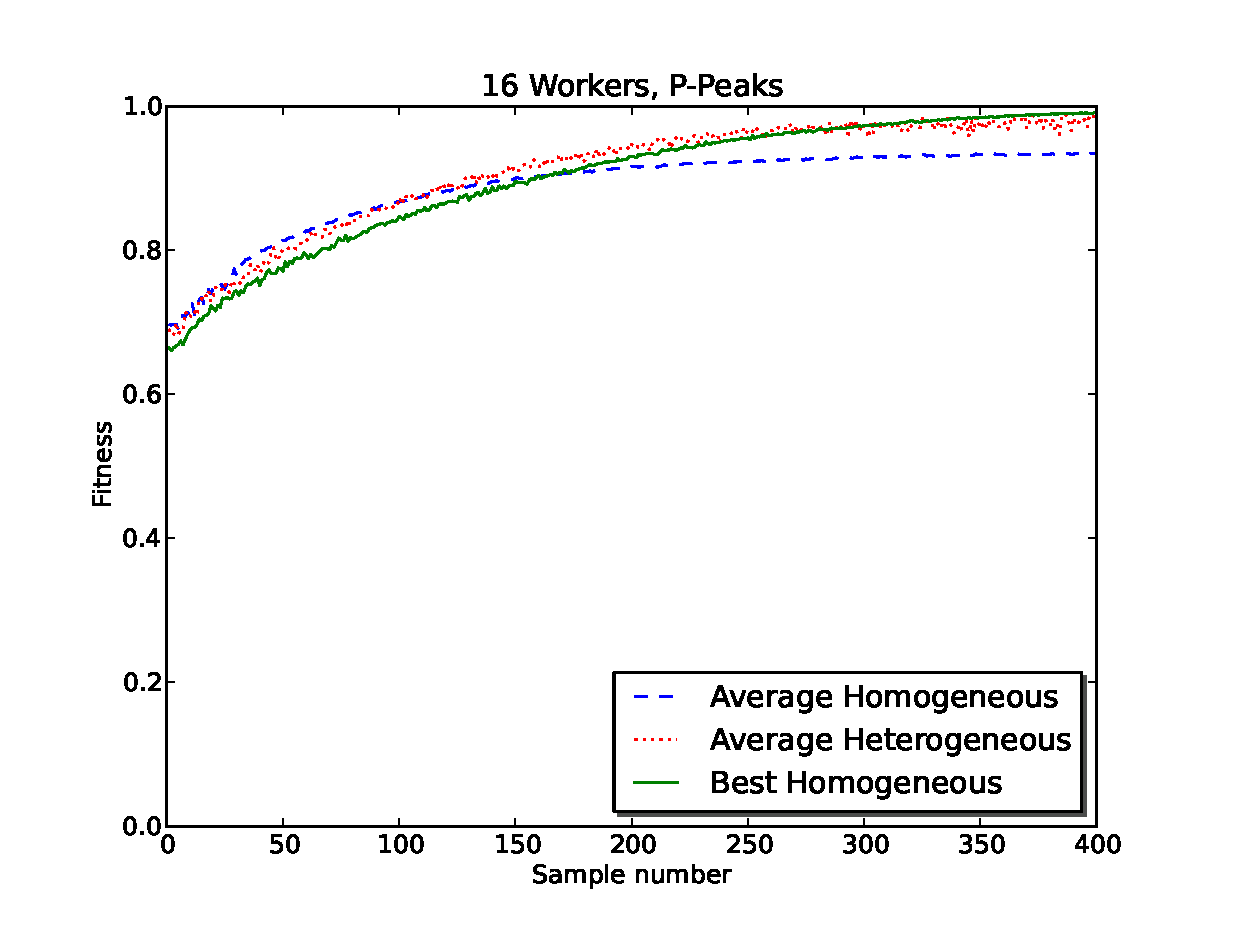
\includegraphics[width=3.5in]{eps/PPeaks-w16.eps}
\caption{Convergence plots for the P-Peaks with 16 EvoWorkers.}
\label{fig:PPeaks-w16}
\end{figure}

\begin{figure}[t]
\centering
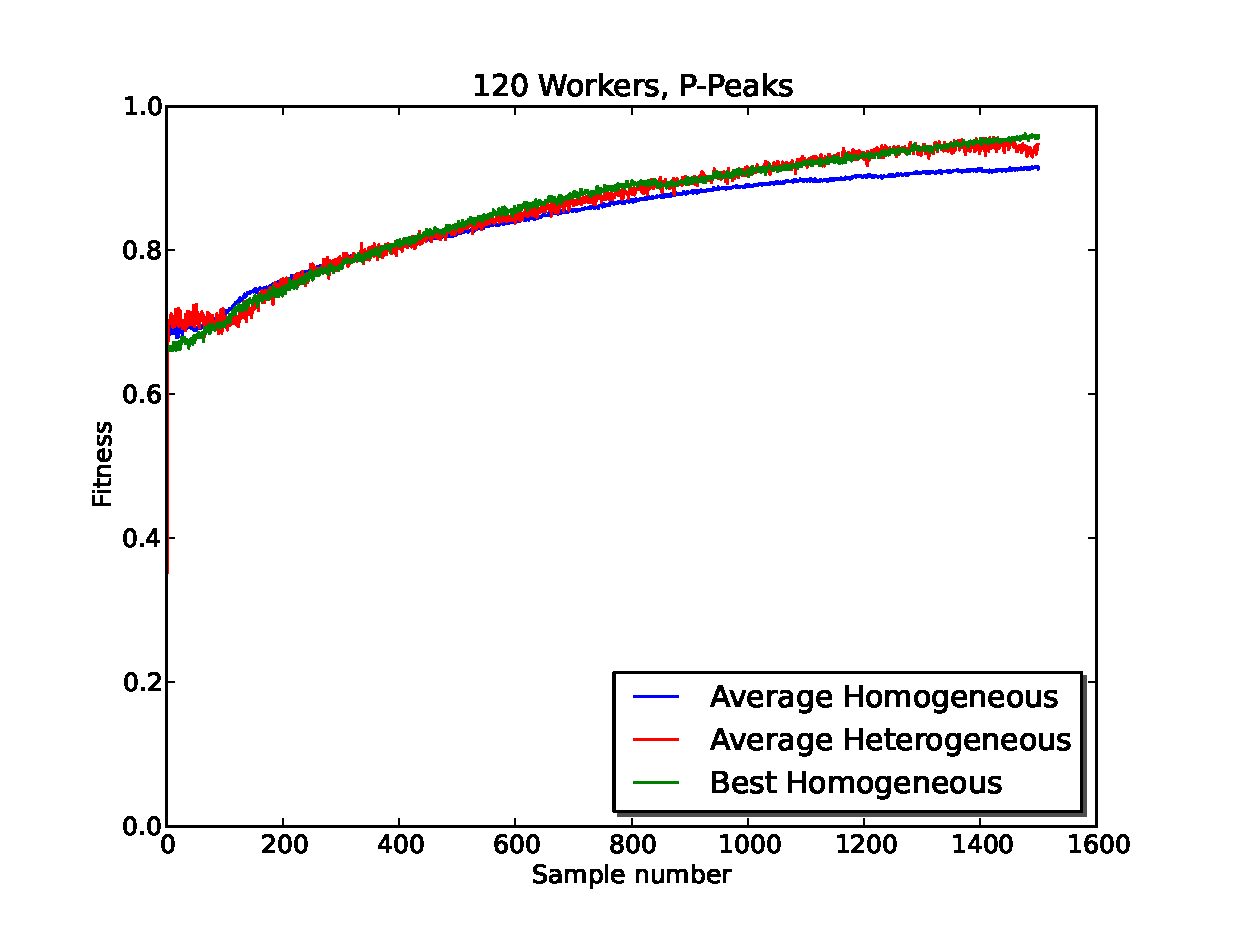
\includegraphics[width=3.5in]{eps/PPeaks-w120.eps}
\caption{Convergence plots for the P-Peaks with 16 EvoWorkers.}
\label{fig:PPeaks-w120}
\end{figure}


First, for the P-Peaks problem with 16 EvoWorkers.
In this case, we can see a clear trend, the random Heterogeneous configuration is very similar with the best homogeneous configuration,
depicted in Figure \ref{fig:PPeaks-w16}.
This is a promising initial observation, since the heterogeneous configuration did not require any parameter tuning, while the best homogeneous configuration
is chosen from a set of 200 runs.
Moreover, we see that using an homogeneous configuration with random values achieves noticeably inferior performance.
When the number of EvoWorkers is increased, shown in Figure \ref{fig:PPeaks-w120}, we see a similar trend,
however the differences among the algorithms are noticeably reduced.
Nevertheless, it is obvious that using a random heterogeneous parametrization can be used as an off-the shelf approach on this problem.


%As EvoSpace is only the population store, EvoWorkers must implement 
%the genetic operators. The genetic algorithm executed by EvoWorkers has been implemented 
%using a modified DEAP (Distributed Evolutionary Algorithms in Python) 
%framework \cite{DEAP_JMLR2012} GA. Is important to note that only the basic non-distributed GA 
%library was used. Three methods were added to the local algorithm: 
%{ \tt  getSample()} and  {\tt putBack()}; and  another for the  initialization 
%of the population. The implementation of the local GA simply uses DEAP´s methods; for instance to 
%generate the initial population, a local {\tt initialize()} is called 
%and the population sent to EvoSpace.
%
%The selection of parameters was based on those used in \cite{Alba:2002dq}: a
%tournament size of 4 individuals, a crossover rate of 0.85 and a
%population of 512 individuals. In  \cite{Jong:PS97} a mutation rate
%equal to the reciprocal of the chromosome length; is recommended, as
%DEAP uses two parameters they were defined as follows, mutation
%probability of 0.5 and an independent flip probability of 0.02. For
%EvoWorkers the parameters were 128 worker generations for each
%sample, and a sample size of 16. To simulate unreliable workers each worker 
%was assigned a return sample probability. In the experiments the lower 
%probability was a 30\% chance of an EvoWorker returning a sample or
%an EvoWorker failing 70\% of the time; other return sample probabilities
%where 50\%, 70\% and 90\%. Experiments where carried out for 4, 
%8 and 16 EvoWorkers. In a pool based  asynchronous GAs there is usually no need 
%to wait for a worker´s job to start a new generation. Although supported by EvoSpace
%time outs were not chosen as triggers to feed the population with new
%individuals, the population size was used instead. We believe the population
%size is a better threshold as it is more critical to the GA performance. 
%In a previous work we found that when the population remaining in the pool 
%was near starvation, the time of completion was increased. For these 
%experiments, the insertion of individuals was triggered when less than 128
%individuals remain in the population; the number of individuals feed to the
%population was 128, or 8 samples when the re-insertion algorithm
%was used. A summary of the setup is presented in table~\ref{params}.
%
%\begin{table}[!t]
%\renewcommand{\arraystretch}{1.3}
%\caption{GA and EvoWorker parameters for experiments.}
%\label{params}
%\centering
%\begin{tabular}{|l|c|}
%\hline
%\multicolumn{2}{|c|}{GA Parameters} \\
%\hline
%Tournament size & 4 \\
%Crossover rate & 0.85  \\
%Population Size & 512 \\
%Mutation probability & 0.5 \\
%Independent bit flip probability  & 0.02 \\
%\hline
%\multicolumn{2}{|c|}{EvoWorker Parameters} \\
%\hline
%Sample Size & 16 \\
%Generations & 128 \\
%\hline
%\multicolumn{2}{|c|}{Other Parameters} \\
%\hline
%PiCloud Worker Type & Realtime \\
%Number of Workers & 4,8,16 \\
%Return Sample Probability & 30\%,50\%,90\% \\
%Number of Executions & 30 \\
%
%\hline
%
%\end{tabular}
%\end{table}


%Quizás deberías poner los random para el mismo número de
%eliminaciones al lado de reinsert, 30, 30, 50, 50 y así
%sucesivamente, sería más fácil compararlos. 
%% Hecho, Mario




%\subsection{Results}
%In this section, results from the experiments are discussed. 
%Figure~\ref{fig:plot_time_ri_w4} shows the time required 
%to solution when using four EvoWorkers. For a population of
%512 individuals and a sample size of 16, there is no
%difference in the time required to solution for 
%percentages of 50\% and above. Both re-insertion algorithms
%had comparable times. For 30 percent, both approaches 
%had slight increase in time. For 8 workers 
%(see Figure~\ref{fig:plot_time_ri_w8})  there was marginal
%decrease in overall time; and results where 
%similar to those found in the experiments with 4 workers.  
%Figure~\ref{fig:plot_time_ri_w16} shows results for 16 workers,
%when there was only a 30\% chance of returning a sample 
%the rate of re-insertions was high, approximately once every 35
%samples. In this case, the insertion of random individuals 
%resulted in a higher time to solution. For these experiments
%when there is not a high rate of re-insertion, both alternatives
%have similar results, but the re-insertion algorithm is better
%for situations when there are many starvation conditions. It appears
%that the insertion of random individuals is not detrimental when there
%are other evolved individuals in the pool. But when the remaining
%pool almost consists of random individuals, samples pulled by
%EvoWorkers need to start the search all over again. 
%If not many samples are then returned to the pool, the work needed to reach an
%optimum is increased. Figure~\ref{fig:plot_evals_w16} also shows the number 
%of evaluations needed to reach an optimum again for 16 workers.
%Figures~\ref{fig:plot_percent_90} and \ref{fig:plot_percent_30} show
%the time required to solution for 30 and 90 percent of returned samples.
%For 90\% both algorithms had similar speedups when incrementing the number of
%workers. The marginal speedup obtained for these experiments is related to 
%the population size, but this parameter was not changed. For 30\% 
%there was practically no speedup at all. The re-insert algorithm
%although not significant, had consistent decrease in time.         
%
%Fitness by time was measured as the average from each consecutive
%sample pulled by each worker. For each sample the average fitness
%was measured at the start and at the end of the local evolution.
%Also the minimum and maximum fitness values at start and finish was 
%recorded. Final fitness values are shown in double width lines in figures.
%Readings used for these figures include all samples, including
%those that where not returned.   
%Figure~\ref{fig:Fitness-w16-30-random} shows fitness by time
%for the random insertion algorithm, as expected initial fitness drops
%at certain points, when random insertion occurs. Average final fitness 
%is affected by random insertions.Figure~\ref{fig:Fitness-w16-30-reinsert}
%shows results for the re-insertion algorithm, with more
%characteristic curves for this type of algorithms. 
% 
 

% Podrías comparar también el resultado para un porcentaje
% determinado, 90 y 30 para todos los números de workers y
% discutirlo. Es presentar los datos de otra forma solamente - JJ
%% Hecho, Mario

% Quizás también presentar como evoluciona el fitness en función del
% tiempo para los dos tipos de reinserciones y para el mínimo y máximo
% porcentaje de reinserción, para que se vea en qué fase del algoritmo
% influye más, principio o final o qué. Yo creo que al principio
% variará poco si es random o reinsertado - JJ 

% Habría que extender más esta sección de resultados y añadir algo de
% discusión. Al final queda un poco débil y va a ser difícil que lo
% admitan como trabajo, sólo como póster. - JJ

\section{Conclusions and Further Work}
\label{sec:conclusions}

%The re-insertion algorithm proposed for EvoSpace is a viable alternative
%to deal with a starving population in pool based GAs, and unreliable EvoWorkers.
%Using  a benchmark problem from the P-Peaks problem generator, 
%the approach was compared against the option of inserting  
%randomly generated individuals. The same parameters and computing resources
%were used when testing both algorithms with better times reported when
%using the proposed technique. For experiments where the population
%size is enough for the number of workers with their sample sizes, plus a 
%buffer to account for loss samples, then both algorithms could be used.
%However for cases when the number of EvoWorkers is unknown an hybrid approach
%could be used, insertion of random individuals to gradually increase the population
%size, and a re-insertion queue to handle lost samples. Further work could be
%focused on a hybrid approach, and also using heterogeneous computing resources. 

\section{Acknowledgments}

Hidden for double-blind review. 

%
% ---- Bibliography ----
% There are problems with the bibliography codification.
\bibliographystyle{abbrv}
\begin{footnotesize}
\bibliography{biblio}
\end{footnotesize}

\end{document}
